% ------------------------------------------------------------------------------
% TYPO3 Version 10.4 - What's New (English Version)
%
% @author	Michael Schams <schams.net>
% @license	Creative Commons BY-NC-SA 3.0
% @link		https://typo3.org/help/documentation/whats-new/
% @language	English
% ------------------------------------------------------------------------------

\section{Introduction}
\begin{frame}[fragile]
	\frametitle{Introduction}

	\begin{center}\huge{Introduction}\end{center}
	\begin{center}\huge{\color{typo3darkgrey}\textbf{The Facts}}\end{center}

\end{frame}

% ------------------------------------------------------------------------------
% TYPO3 Version 10.4 - The Facts

\begin{frame}[fragile]
	\frametitle{Introduction}
	\framesubtitle{TYPO3 Version 10.4 - The Facts}

	\begin{itemize}
		\item Release date: 21 April 2020
		\item Release type: LTS (Long-term Support)
	\end{itemize}

	\begin{figure}
		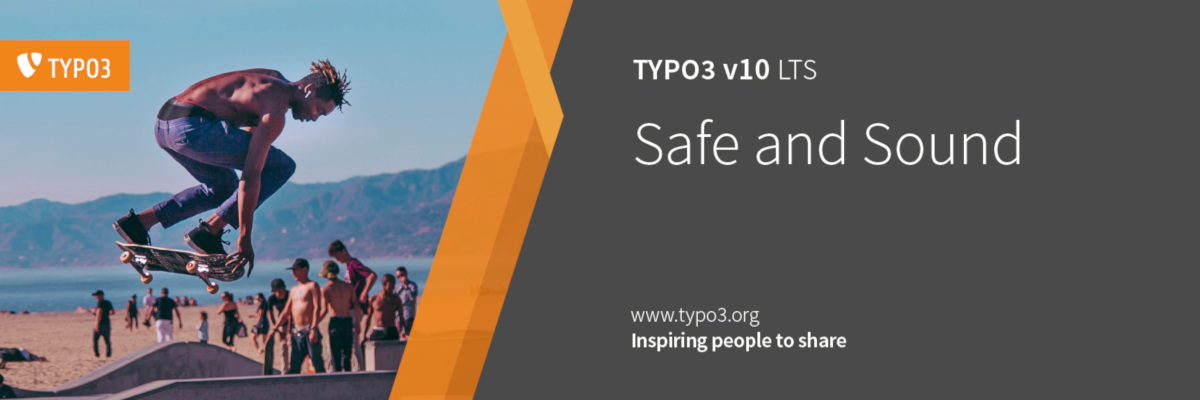
\includegraphics[width=0.95\linewidth]{Introduction/typo3-v10-4-banner.jpg}
	\end{figure}

\end{frame}

% ------------------------------------------------------------------------------
% TYPO3 Version 10.4 - Executive Summary

\begin{frame}[fragile]
	\frametitle{Introduction}
	\framesubtitle{Executive Summary}

	\small
		TYPO3 v10.4 (also called TYPO3 v10 LTS indicating this is a long-term support version)
		is our new flagship and, without doubt, one of the most advanced PHP-based open-source
		content management systems on the market to date.

		\vspace{0.2cm}

		After publishing five sprint releases since July 2019, we can proudly claim that we
		have equipped TYPO3 with the top modern PHP libraries and that we have introduced some
		fantastic new enterprise features.

		\vspace{0.2cm}

		Please note that this document summarizes the changes between TYPO3 v10.3 and v10.4 only.

		\vspace{0.2cm}

		"What's New Slides" of all TYPO3 v10.x releases are available at
		\href{https://typo3.org/help/documentation/whats-new/}{typo3.org}.

	\normalsize

\end{frame}

% ------------------------------------------------------------------------------
% System Requirements

\begin{frame}[fragile]
	\frametitle{Introduction}
	\framesubtitle{System Requirements}

	\begin{itemize}
		\item PHP version 7.2, 7.3 or 7.4
		\item PHP settings:

			\begin{itemize}
				\item \texttt{memory\_limit} >= 256M
				\item \texttt{max\_execution\_time} >= 240s
				\item \texttt{max\_input\_vars} >= 1500
				\item compilation option \texttt{-}\texttt{-disable-ipv6} must \underline{not} be used
			\end{itemize}

		\item Most database servers supported by \textbf{Doctrine DBAL} also work with TYPO3.
			Tested DB engines are for example:
	\end{itemize}

	\begin{figure}
		
\includegraphics[width=0.80\linewidth]{Introduction/logo-databases.png}
	\end{figure}

\end{frame}

% ------------------------------------------------------------------------------
% Development, Release, and Maintenance Timeline

\begin{frame}[fragile]
	\frametitle{Introduction}
	\framesubtitle{Development, Release, and Maintenance Timeline}

	\textbf{TYPO3 v10}

	\begin{figure}
		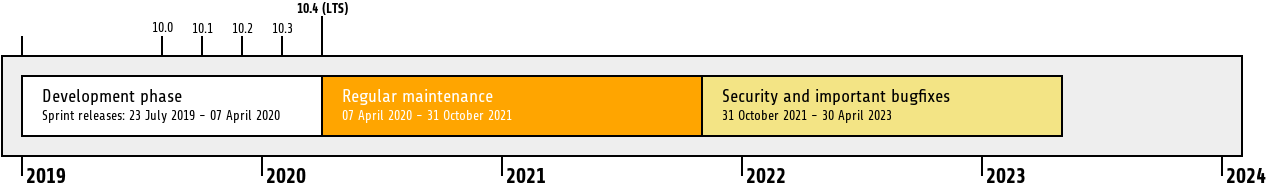
\includegraphics[width=1\linewidth]{Introduction/typo3-v10-lifecycle.png}
	\end{figure}

	\textbf{Extended Support}\newline
	\smaller
		The \href{https://typo3.com}{TYPO3 GmbH} offers further support options
		for TYPO3 v10 LTS even after 30 April 2023 for up to three additional
		years.
	\normalsize

\end{frame}

% ------------------------------------------------------------------------------
% TYPO3 v10 Roadmap

\begin{frame}[fragile]
	\frametitle{Introduction}
	\framesubtitle{TYPO3 v10 Roadmap}

	Release dates and their primary focus:

	\begin{itemize}

		\item v10.0 \tabto{1.1cm}23/July/2019\tabto{3.4cm}Pave the way for exciting new concepts and APIs
		\item v10.1 \tabto{1.1cm}01/Oct/2019\tabto{3.4cm}Routing Improvements and Site Handling v2
		\item v10.2 \tabto{1.1cm}03/Dec/2019\tabto{3.4cm}Fluid/Rendering Engine Improvements
		\item v10.3 \tabto{1.1cm}25/Feb/2020\tabto{3.4cm}Feature Freeze
		\item
			\begingroup
				\color{typo3orange}
				v10.4 \tabto{1.1cm}21/Apr/2020\tabto{3.4cm}LTS Release (long-term support)
			\endgroup

	\end{itemize}

	\vspace{0.6cm}
	\smaller
		\url{https://typo3.org/article/typo3-v10-roadmap}\newline
		\url{https://typo3.org/article/typo3-v10-lts-safe-and-sound}
	\normalsize

\end{frame}

% ------------------------------------------------------------------------------
% Installation

\begin{frame}[fragile]
	\frametitle{Introduction}
	\framesubtitle{Installation}

	\begin{itemize}
		\item Official \textit{classic} installation procedure under Linux/Mac OS X\newline
			(DocumentRoot for example \texttt{/var/www/site/htdocs}):
\begin{lstlisting}
$ cd /var/www/site
$ wget --content-disposition get.typo3.org/10.4
$ tar xzf typo3_src-10.4.0.tar.gz
$ cd htdocs
$ ln -s ../typo3_src-10.4.0 typo3_src
$ ln -s typo3_src/index.php
$ ln -s typo3_src/typo3
$ touch FIRST_INSTALL
\end{lstlisting}

		\item Symbolic links under Microsoft Windows:

			\begin{itemize}
				\item Use \texttt{junction} under Windows XP/2000
				\item Use \texttt{mklink} under Windows Vista and Windows 7 and higher
			\end{itemize}

	\end{itemize}
\end{frame}

% ------------------------------------------------------------------------------
% Installation using composer

\begin{frame}[fragile]
	\frametitle{Installation and Upgrade}
	\framesubtitle{Installation Using \texttt{composer}}

	\begin{itemize}
		\item Installation using \textit{composer} under Linux, Mac OS X and Windows 10:
\begin{lstlisting}
$ cd /var/www/site/
$ composer create-project typo3/cms-base-distribution typo3v10 ^10.4
\end{lstlisting}

		\item Alternatively, create your custom \texttt{composer.json} file and run:
\begin{lstlisting}
$ composer install
\end{lstlisting}

			Further details about Composer for the TYPO3 core and for TYPO3 extensions
			are available at:

			\small
				\href{https://get.typo3.org/misc/composer/repository}{https://get.typo3.org/misc/composer/repository}
			\normalsize

	\end{itemize}
\end{frame}

% ------------------------------------------------------------------------------
